% allgem. Dokumentenformat
\documentclass[a4paper,12pt,headsepline]{scrartcl}
%Variablen welche innerhalb der gesamten Arbeit zur Verfügung stehen sollen
\newcommand{\titleDocument}{Bachelor Thesis}
\newcommand{\subjectDocument}{in Computer Science}


\newcommand{\specialcell}[2][c]{%
	\begin{tabular}[#1]{c}
		#2
	\end{tabular}
}

\newcommand{\specialcellleft}[2][@{}l]{%
	\begin{tabular}[#1]{@{}l}
		#2
	\end{tabular}
}

\newcommand{\fixme}[1]{
	~\\
	\noindent
	\textbf{\textcolor{red}{FIXME: #1}}
	\\
}




% weitere Pakete
% Grafiken aus PNG Dateien einbinden
\usepackage{graphicx}

% Eurozeichen einbinden
\usepackage[right]{eurosym}

% Umlaute unter UTF8 nutzen
\usepackage[utf8]{inputenc}

% Zeichenencoding
\usepackage[T1]{fontenc}

\usepackage{lmodern}
\usepackage{fix-cm}

% floatende Bilder ermöglichen
%\usepackage{floatflt}

% mehrseitige Tabellen ermöglichen
\usepackage{longtable}

% Unterstützung für Schriftarten
%\newcommand{\changefont}[3]{ 
%\fontfamily{#1} \fontseries{#2} \fontshape{#3} \selectfont}

% Packet für Seitenrandabständex und Einstellung für Seitenränder
\usepackage{geometry}
\geometry{left=3.5cm, right=2cm, top=2.5cm, bottom=2cm}

% Paket für Boxen im Text
\usepackage{fancybox}

% bricht lange URLs "schoen" um
\usepackage[hyphens,obeyspaces,spaces]{url}

% Paket für Textfarben
\usepackage{color}

% Mathematische Symbole importieren
\usepackage{amssymb}

% auf jeder Seite eine Überschrift (alt, zentriert)
%\pagestyle{headings}

% erzeugt Inhaltsverzeichnis mit Querverweisen zu den Kapiteln (PDF Version)
\usepackage[bookmarksnumbered,pdftitle={\titleDocument},hyperfootnotes=false]{hyperref} 
%\hypersetup{colorlinks, citecolor=red, linkcolor=blue, urlcolor=black}
%\hypersetup{colorlinks, citecolor=black, linkcolor= black, urlcolor=black}

% neue Kopfzeilen mit fancypaket
\usepackage{fancyhdr} %Paket laden
\pagestyle{fancy} %eigener Seitenstil
\fancyhf{} %alle Kopf- und Fußzeilenfelder bereinigen
\fancyhead[L]{\nouppercase{\leftmark}} %Kopfzeile links
\fancyhead[C]{} %zentrierte Kopfzeile
\fancyhead[R]{\thepage} %Kopfzeile rechts
\renewcommand{\headrulewidth}{0.4pt} %obere Trennlinie
%\fancyfoot[C]{\thepage} %Seitennummer
%\renewcommand{\footrulewidth}{0.4pt} %untere Trennlinie

% für Tabellen
\usepackage{array}

% Runde Klammern für Zitate
%\usepackage[numbers,round]{natbib}

% Festlegung Art der Zitierung - Havardmethode: Abkuerzung Autor + Jahr
\bibliographystyle{alphadin}

% Schaltet den zusätzlichen Zwischenraum ab, den LaTeX normalerweise nach einem Satzzeichen einfügt.
\frenchspacing

% Paket für Zeilenabstand
\usepackage{setspace}

% für Bildbezeichner
\usepackage{capt-of}

% für Stichwortverzeichnis
\usepackage{makeidx}

% für Listings
\usepackage{listings}
\lstset{numbers=left, numberstyle=\tiny, numbersep=5pt, keywordstyle=\color{black}\bfseries, stringstyle=\ttfamily,showstringspaces=false,basicstyle=\footnotesize,captionpos=b}
\lstset{language=java}

% Indexerstellung
\makeindex

% Abkürzungsverzeichnis
\usepackage[english]{nomencl}
\let\abbrev\nomenclature

% Abkürzungsverzeichnis LiveTex Version
\renewcommand{\nomname}{Abbreviations}
\setlength{\nomlabelwidth}{.25\hsize}
\renewcommand{\nomlabel}[1]{#1 \dotfill}
\setlength{\nomitemsep}{-\parsep}
\makenomenclature
%\makeglossary

% Abkürzungsverzeichnis TeTEX Version
% \usepackage[german]{nomencl}
% \makenomenclature
% %\makeglossary
% \renewcommand{\nomname}{Abkürzungsverzeichnis}
% \setlength{\nomlabelwidth}{.25\hsize}
% \renewcommand{\nomlabel}[1]{#1 \dotfill}
% \setlength{\nomitemsep}{-\parsep}

% Disable single lines at the start of a paragraph (Schusterjungen)
\clubpenalty = 10000
% Disable single lines at the end of a paragraph (Hurenkinder)
\widowpenalty = 10000
\displaywidowpenalty = 10000

\begin{document}
% hier werden die Trennvorschläge inkludiert
%hier müssen alle Wörter rein, welche Latex von sich auch nicht korrekt trennt bzw. bei denen man die genaue Trennung vorgeben möchte
\hyphenation{
Film-pro-du-zen-ten
Lux-em-burg
Soft-ware-bau-steins
zeit-in-ten-siv
}

%Schriftart Helvetica
%\changefont{phv}{m}{n}

% Leere Seite am Anfang
\newpage
\thispagestyle{empty} % erzeugt Seite ohne Kopf- / Fusszeile
\section*{ }

% Titelseite %
% das Papierformat zuerst
%\documentclass[a4paper, 11pt]{article}

% deutsche Silbentrennung
%\usepackage[ngerman]{babel}

% wegen deutschen Umlauten
%\usepackage[ansinew]{inputenc}

% hier beginnt das Dokument
%\begin{document}


\thispagestyle{empty}

%\begin{figure}[t]
% \includegraphics[width=0.6\textwidth]{abb/fh_koeln_logo}
%\end{figure}

\begin{figure}[t]
 \centering
 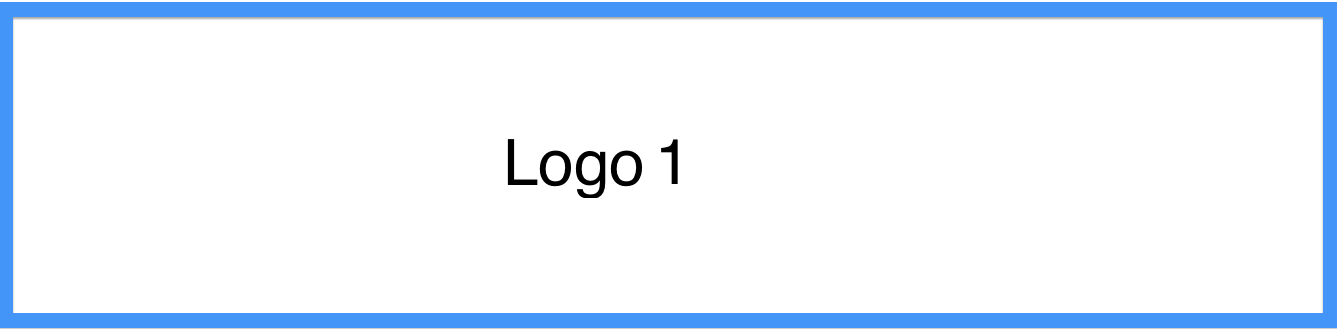
\includegraphics[width=0.6\textwidth]{abb/logo1}
~~~~~~~~~~
 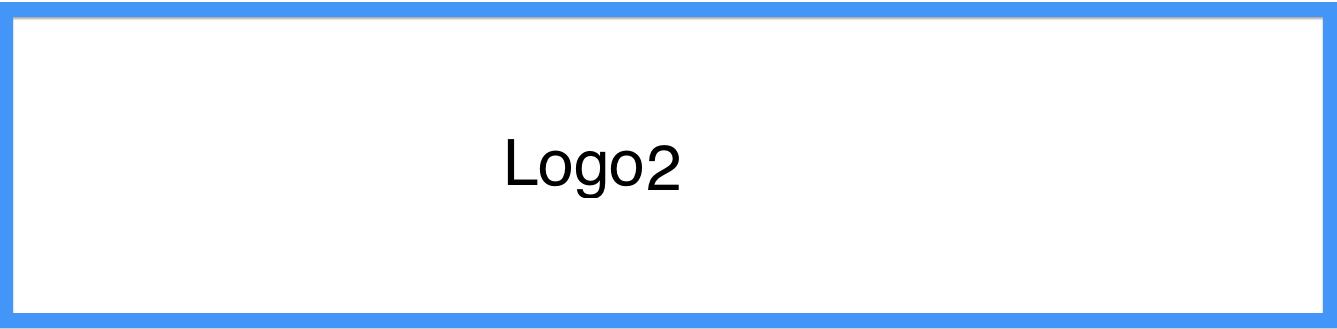
\includegraphics[width=0.20\textwidth]{abb/logo2}
\end{figure}


\begin{verbatim}


\end{verbatim}

\begin{center}
\Large{University of Bayreuth}\\
\end{center}


\begin{center}
\Large{Institute for Computer Science}
\end{center}
\begin{verbatim}








\end{verbatim}
\begin{center}
\doublespacing
\textbf{\LARGE{\titleDocument}}\\
\singlespacing
\begin{verbatim}

\end{verbatim}
\textbf{{~\subjectDocument}}
\end{center}
\begin{verbatim}

\end{verbatim}
\begin{center}

\end{center}
\begin{verbatim}






\end{verbatim}
\begin{flushleft}
\begin{tabular}{llll}
\textbf{Topic:} & & Integration of JPA-conform ORM-Implementations & \\
	& & in Hibernate Search & \\
& & \\
\textbf{Author:} & & Martin Braun <martinbraun123@aol.com>& \\
& & Matrikel-Nr. 1249080 & \\
& & \\
\textbf{Version date:} & & \today &\\
& & \\
\textbf{1. Supervisor:} & & Prof. Dr. Stefan Jablonski &\\
\textbf{2. Supervisor:} & & Prof. Dr. Bernhard Westfechtel &\\
\end{tabular}
\end{flushleft}
%
%\pagebreak
%~
%\pagebreak

%\begin{verbatim}






















%\end{verbatim}

%\begin{center}
%	To my parents.
%\end{center}

%\afterpage{\null\newpage}
%\pagebreak
%~\\\\
%\pagebreak
%~

% römische Numerierung
%\pagenumbering{arabic}

% 1.5 facher Zeilenabstand
\onehalfspacing

% Einleitung / Abstract
% !TeX spellcheck = en_GB
\section*{Abstract}

Fulltext search engines are a powerful tool to improve query results in applications where relational databases don't suffice. However, they don't integrate well with the widely spread concept of object relationship mappers (ORM, in Java predominantly represented by the standard JPA) in the object oriented programming world.
\\\\
This is where Hibernate Search comes into use for Java developers: It combines JPA and fulltext search by being the intermediary between Hibernate ORM and a Lucene based fulltext index. It has one problem though: Hibernate Search only works with Hibernate ORM but not with other JPA-conform providers even though it is possible to support these. In this thesis we will show how such a generic version can be accomplished.
\\\\
After discussing the methods we use, we give an explanation why a generic Hibernate Search is a desirable solution for JPA developers. Creating it is challenging as we have to build a standalone version of Hibernate Search's internal engine first and then integrate it with JPA together with an automatic index updating mechanism. We solve these challenges and give a usage example of the completed generic version. Finally, we discuss the current development state of the generic version and give an outlook on the planned merging process with the original Hibernate Search.

\pagebreak

\section*{Zusammenfassung}
Volltextsuchengines sind ein wertvolles Werkzeug um Suchergebnisse in Anwendungen zu verbessern, wenn relationale Datenbanken nicht ausreichen. Diese Engines sind jedoch nicht gut mit dem in der objekt-orientierten Programmierungs-Welt weit verbreiteten Konzept der Objekt-Relationalen Mapper (ORM, in Java vor allem durch den Standard JPA repräsentiert) integriert. 
\\\\
Für Java Entwickler bietet hier Hibernate Search eine Abhilfe: Es kombiniert JPA und Volltextsuche und stellt die Schnittstelle zwischen Hibernate ORM und einem Lucene basierten Volltextindex dar. Es hat aber ein Problem: Hibernate Search funktioniert nur in Kombination mit Hibernate ORM, aber nicht mit anderen JPA konformen Providern, obwohl es möglich wäre diese zu unterstützen. In dieser Thesis wird daher gezeigt, wie eine solche generische Version realisiert werden kann.
\\\\
Nachdem die benutzten Methoden erklärt wurden, wird eine Begründung dafür gegeben, warum Hibernate Search eine wünschenswerte Lösung für JPA Entwickler ist. Diese zu entwickeln ist eine Herausforderung, da wir zuerst eine Standalone Version von Hibernate Search's interner Engine bauen müssen, um diese danach in eine JPA Version zusammen mit einem automatischen Index Updating Mechanismus zu integrieren. Wir zeigen wie diese Probleme gelöst werden und erklären die Benutzung anhand eines Beispiels. Zuletzt gehen wir auf den aktuellen Entwicklungsstand der generischen Version ein und geben einen Ausblick auf den geplanten Merge-Prozess mit dem originalen Hibernate Search.



% einfacher Zeilenabstand
\singlespacing

% Inhaltsverzeichnis anzeigen
\newpage
\tableofcontents

% das Abbildungsverzeichnis
%\newpage
% Abbildungsverzeichnis soll im Inhaltsverzeichnis auftauchen
%\addcontentsline{toc}{section}{List of figures}
% Abbildungsverzeichnis endgueltig anzeigen
%\listoffigures

% das Tabellenverzeichnis
%\newpage
% Abbildungsverzeichnis soll im Inhaltsverzeichnis auftauchen
%\addcontentsline{toc}{section}{Tabellenverzeichnis}
% \fancyhead[L]{Abbildungsverzeichnis / Abkürzungsverzeichnis} %Kopfzeile links
% Abbildungsverzeichnis endgueltig anzeigen
%\listoftables

%% WORKAROUND für Listings
%\makeatletter% --> De-TeX-FAQ
%\renewcommand*{\lstlistoflistings}{%
%  \begingroup
%    \if@twocolumn
%      \@restonecoltrue\onecolumn
%    \else
%      \@restonecolfalse
%    \fi
%    \lol@heading
%    \setlength{\parskip}{\z@}%
%    \setlength{\parindent}{\z@}%
%    \setlength{\parfillskip}{\z@ \@plus 1fil}%
%    \@starttoc{lol}%
%    \if@restonecol\twocolumn\fi
%  \endgroup
%}
%\makeatother% --> \makeatletter
% das Listingverzeichnis
%\newpage
% Listingverzeichnis soll im Inhaltsverzeichnis auftauchen
%\addcontentsline{toc}{section}{Listingverzeichnis}
%\fancyhead[L]{Abbildungs- / Tabellen- / Listingverzeichnis} %Kopfzeile links
%\renewcommand{\lstlistlistingname}{Listingverzeichnis}
%\lstlistoflistings
%%%%

% das Abkürzungsverzeichnis
%\newpage
% Abkürzungsverzeichnis soll im Inhaltsverzeichnis auftauchen
%\addcontentsline{toc}{section}{Abkürzungsverzeichnis}
% das Abkürzungsverzeichnis entgültige Ausgeben
%\fancyhead[L]{Abkürzungsverzeichnis} %Kopfzeile links
%\nomenclature{UGC}{User Generated Content}
\nomenclature{CSS}{Cascading Style Sheets}
\nomenclature{JS}{JavaScript}
\nomenclature{SQL}{Structured Query Language}
\nomenclature{GPL}{GNU General Public License}
\nomenclature{GNU}{GNU is not Unix}
\nomenclature{LGPL}{GNU Lesser General Public License}
\nomenclature{XMPP}{Extensible Messaging and Presence Protocol}
\nomenclature{IM}{Instant Message}
\nomenclature{CMS}{Content Management System}
\nomenclature{RSS}{Really Simple Syndication}
\nomenclature{JSON}{JavaScript Object Notation}
\nomenclature{HTML}{Hypertext Markup Language}
\nomenclature{TDD}{Test-driven development}
\nomenclature{GUI}{Graphical User Interface}
\nomenclature{KPI}{Key Performance Indicator}
\nomenclature{WWW}{World Wide Web}
\nomenclature{OCR}{Optical Character Recognition}
\nomenclature{ERM}{Entity Relationship Modell}

%\printnomenclature

% Definiert Stegbreite bei zweispaltigem Layout
\setlength{\columnsep}{25pt}

%%%%%%% EINLEITUNG %%%%%%%%%%%%
%\twocolumn
\newpage
\fancyhead[L]{\nouppercase{\leftmark}} %Kopfzeile links

% 1,5 facher Zeilenabstand
\onehalfspacing










% einzelne Kapitel
% !TeX spellcheck = en_GB

\section{Preface}\label{Preface}
In the software world, or more specific, the Java enterprise world, developers tend to abstract access to data in a way that components are interchangeable. A perfect example for such an abstraction is the usage of Object Relational Mappers (ORM). The database specifics are mostly uninteresting to the average developer and the need for native SQL is brought down to a minimum. This makes the switch to a different relational database system (RDBMS) easier in the later stages of a product's life cycle.
\\\\
The Java Persistence API (JPA) went even further by providing a standard for ORMs. First conceived in 2006 as part of EJB 3.0 \footnote{JSR 220: Enterprise Java Beans 3.0, see~\cite{jsr_jpa1}} \footnote{Javaworld: Understanding JPA, Part 1, see~\cite{javaworld_jpa1}}, it is now the de-facto standard for Object Relational Mappers in Java. The developer doesn't need to know which specific ORM is used in the application, as all the database queries are written against a standardized query API and are therefore portable. This means that not only the database is interchangeable, but even the specific ORM, it is accessed by, is as well.
\\\\
However, this does not mean that all JPA implementations come with the same features. While all of them are JPA compliant (apart from minor bugs), some ship with additional modules to enhance their capabilities. A perfect example for this is the Hibernate Search API aimed at Hibernate ORM users.\footnote{Hibernate ORM project homepage, see~\cite{hibernate_orm}} \footnote{Hibernate Search project homepage, see~\cite{hibernate_search_homepage}}
\\\\

\pagebreak
\noindent
Nowadays, even small applications like online shops need enhanced search capabilities to let the user find more results for a given input.
This is not something a regular RDBMS excels at and Hibernate Search comes into use as shown in figure \ref{fig1}: It works atop the Hibernate ORM, a popular JPA implementation, and enables the developer to index the domain model for searching. It's not only a mapper from JPA entities to a search index, but also keeps the index up-to-date if something in the database changes.
\\
\begin{figure}[ht]
	\centering
	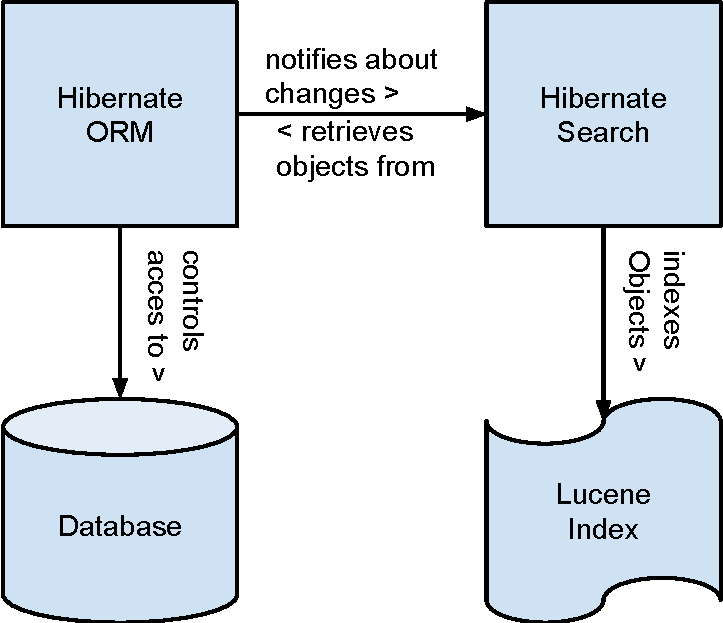
\includegraphics[scale=0.45]{images/hibernate_search_hibernate_schema.pdf}
	\caption{Hibernate Search with Hibernate ORM}
	\label{fig1}
\end{figure}
\\
Hibernate Search is based on the powerful Lucene search toolbox \footnote{sourcecode on Hibernate Search GitHub, see~\cite{hsearch_source_code_git}} \footnote{Hibernate Search FAQ, see~\cite{hibernate_search_faq}} and is a separate project in the Hibernate family and aims to provide a JPA "feeling" in its API as it also incorporates a lot of JPA interfaces in its codebase. However, this does not mean that it is compatible with other JPA providers than Hibernate ORM (apart from Hibernate OGM, the NoSQL JPA mapper of the family) as the following figure \ref{fig2} shows.
\\\\
\begin{figure}[ht]
	\centering
	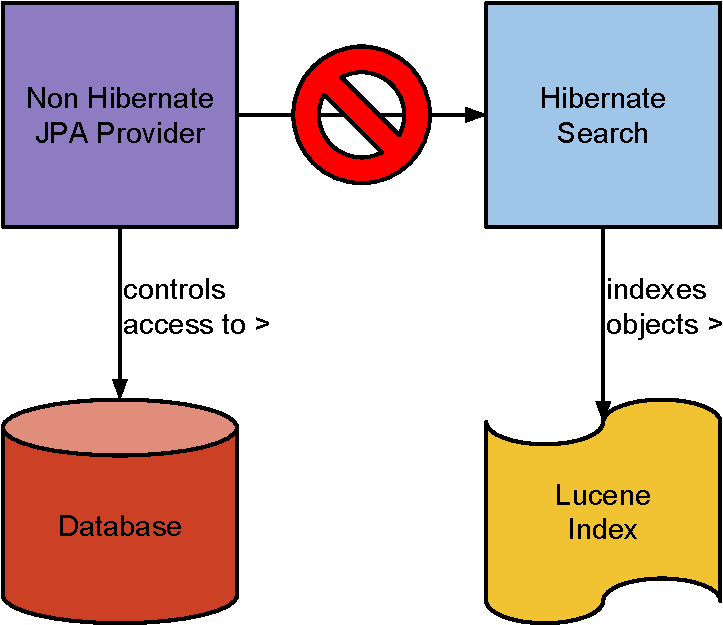
\includegraphics[scale=0.45]{images/hibernate_search_any_jpa_problem_schema.pdf}
	\caption{Hibernate Search's incompatibility with other JPA implementations}
	\label{fig2}
\end{figure}
\\
While using Hibernate Search obviously is beneficial for Hibernate ORM applications, not all developers can bind themselves to a specific JPA implementation in their application. For some, the ability to change implementations might be of strategic importance, for others it could just be sheer preference to use a different JPA implementation.

\noindent
Currently, developers that do not want to bind themselves to Hibernate ORM have to resort to using different full text search systems like native Lucene\footnote{official Lucene website, see~\cite{lucene_apache_org}}, ElasticSearch\footnote{ElasticSearch Java API, see~\cite{elasticsearch_java_api}} or Solr\footnote{Solr Java API, see~\cite{solr_java_api}}. While this is always a viable option, for some applications Hibernate Search would be a much better suit because of its design with a entity structure in mind and the automatic index updating feature, if it just were compatible with generic JPA.
\\\\
When investigating Hibernate Search's project structure
\footnote{Hibernate Search GitHub repository, see~\cite{hsearch_source_code_git}}, we can see that the only module apart from some server-integration modules that depends on any ORM logic is "hibernate-search-orm". The modules that contain the indexing engine, the replication logic, alternative backends, etc. are completely independent from any ORM logic. This means, that most of the codebase could be reused for a generic version of Hibernate Search.
\\\\
\noindent
Creating such a generic Hibernate Search is a better approach for a search API on top of JPA rather than rewriting a JPA binding from scratch. Hibernate Search could then act as an all-purpose API for fulltext search in the JPA world instead of having a competing API that would just do the same thing in a different style.
\\
\begin{figure}[ht]
	\centering
	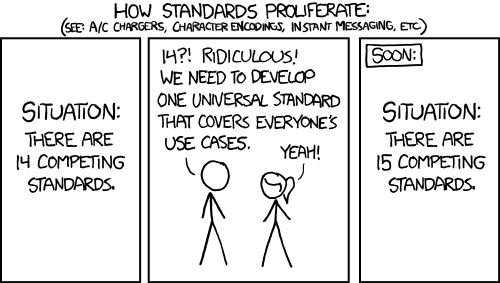
\includegraphics[scale=0.5]{images/competing_standards.png}
	\caption{xkcd.com on competing standards \protect\footnotemark}
	\label{xkcd_standards_fig}
\end{figure}
\footnotetext{xkcd comic \#927, see~\cite{xkcd_competing_standards_source}}
\\
This is why we will show how such a generic version can be built in this thesis. First, we will look at how Hibernate Search's engine can be reused. Then, we will write a standalone version of this engine and finally integrate it with generic JPA.

\pagebreak

\noindent
\textbf{Short overview of contents}:
\\\\
\noindent
In chapter \ref{Methods} we explain what methods we are using to build Hibernate Search GenericJPA. In chapter \ref{Overview} we give an overview over the relevant technologies used in this thesis and give short introductions to several fulltext search engines and the reasoning behind Hibernate Search GenericJPA. In chapter \ref{Challenges} we introduce a small example project and explain the main challenges while developing Hibernate Search GenericJPA. In chapter \ref{standalone_chapter} we describe a standalone version of Hibernate Search. In chapter \ref{integration_jpa} we explain how the JPA integration of the standalone version is designed. In chapter \ref{automatic_indexing_chapter} we work out an automatic index updating mechanism for Hibernate Search GenericJPA. In chapter \ref{usage_chapter} we give a full explanation of how to use Hibernate Search GenericJPA using the example from chapter \ref{Challenges}. In chapter \ref{outlook} we give a summary of we have achieved in this thesis and describe further steps.

\pagebreak

\pagebreak

\section{Methods} \label{Methods}

While developing the generic version of Hibernate Search we are using the following process schema to find the solutions for the all the different problems:

\begin{figure}[ht]
	\centering
	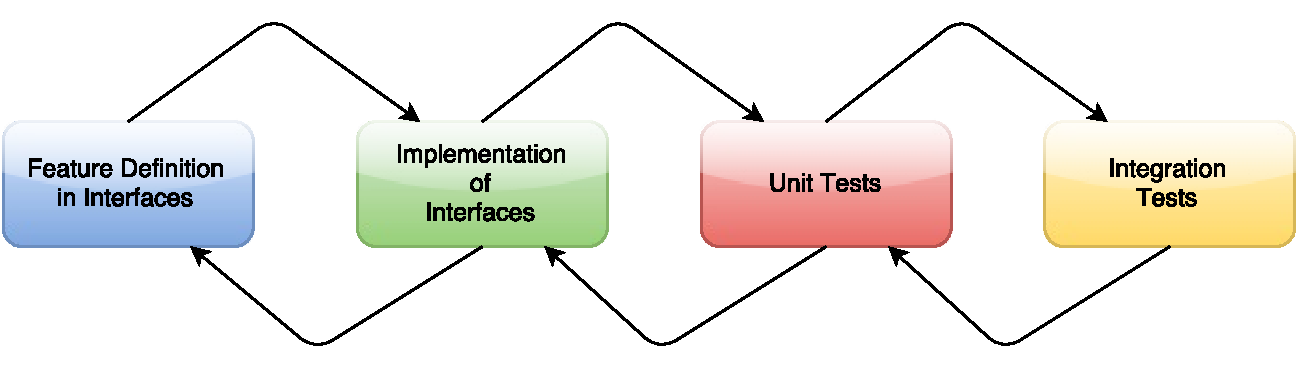
\includegraphics[scale=0.52]{images/work_process.pdf}
	\caption{Development Process}
	\label{development_process_of_a_feature}
\end{figure}

\begin{itemize}
	\item \textbf{Requirements Engineering}: As part of the solution finding process for each problem, we start by specifying a requirements specification that consists of:
	\begin{itemize}
		\item "a specification of the context in which the system will operate,
		\item a list of desired system functions of the system,
		\item a definition of the semantics of these functions,
		\item and a list of quality attributes of those functions" \footnote{Web Engineering, chapter: Requirements Engineering: Problem Analysis and Solution Specification, R. J. Wieringa, 2004, see~\cite{requirements_engineering}}
	\end{itemize}
	While 
	\item \textbf{Feature Definition in Interfaces}: As the next step, the requirements are translated into Java interfaces.	While modelling the interfaces we try to be as compliant to the \textbf{Single Responsibility Principle} \footnote{objectmentor.com: Article on Single Responsibility Principle, see~\cite{singleresponsibility_objectmentor}} as possible because it enforces structures that are easy to reuse and change due to being pluggable single purpose classes. However we explicitly break it in some cases to allow more user-friendly interfaces (mostly in API entry-points).
	\\
	By defining the features in interfaces and using them instead of implementations to write code, we achieve complete independence between the implementing classes and are compliant to the \textbf{Open-Closed-Principle} \footnote{	objectmentor.com: Article on Open-Closed-Principle, see~\cite{openclosed_objectmentor}} internally ("Modules should be both open (for extension) and closed (for modification)" \footnote{Object-Oriented Software Construction, Prentice Hall, 1988, Bertrand Meyer, see~\cite{openclosed_bertrand}}) which allows us to write more "pluggable" code.
	\item \textbf{Implement Interfaces}: Once the interfaces are properly defined, we write implementations for these according to the contracts set. These classes generally don't use other implementations directly and build functionality only by using interfaces.
	\item \textbf{Unit Test}: Each feature has to have a corresponding unit test. These are necessary to test each implementation for the right behaviour (outputs and side-effects) for at least one given input. They also help to identify bugs in the implementations.
	\item \textbf{Integration Test}: While Unit-Tests check the behaviour of every \textit{single} feature implementation, integration tests are used to cover the correct behaviour when used together with the other parts of the project. With these tests we ensure all features interoperate properly with each other.
\end{itemize}
\noindent
Note that once a step is finished, that doesn't mean it is final. As we can see in the diagram, we can go back and forth between the different steps at will to adapt to specific implementation problems and new problems that have not been covered before.
\\\\
We choose this kind of on-the-fly structure because it suits the project best: We have to investigate different approaches before we can work out the real solution, first. Additionally, because "hibernate-search-engine" is an internal API, we have to be as flexible as possible with our development since some features of it can be different than what we might expect in the first place.
\\\\
It is worth mentioning that all the tests (including the integration tests) are executed during each build to ensure no regression bugs occur. This is automatically managed by the Maven \footnote{Maven project homepage, see~\cite{maven_homepage}} build tool.
\\\\
This process is embedded in a combined approach of \textbf{top-down} \footnote{Top-down programming, Robert Strandh, see~\cite{top_down_strandh}} and \textbf{bottom-up} \footnote{Bottom-up programming, Robert Strandh, see~\cite{bottom_up_strandh}} to software development: After dividing the project into submodules (top-down) we develop the building blocks first and integrate them into bigger mechanisms (the sub-modules) as the project goes on (bottom-up). This way we stay flexible in the early stages of development and only have to write "wiring code" in the later stages.

\pagebreak


\section{Showcase of basic Hibernate Search}

%....

\section{Ausblick}\label{ausblick}

\section{Fazit}\label{fazit}

% Beispiel für Bild mit Fußnote
%\begin{figure}[htb]
% \centering
% 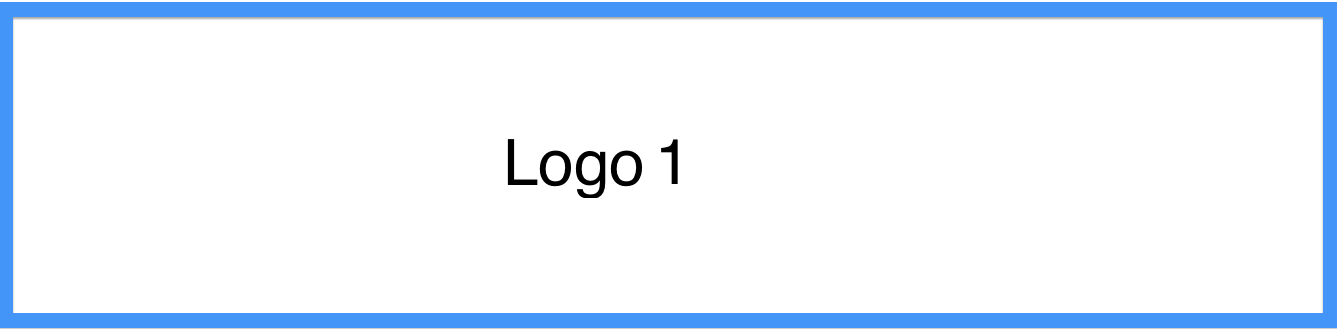
\includegraphics[width=0.4\textwidth,angle=45]{abb/logo1}
% \caption[Beispiel einer Bildbeschreibung]{Beispiel einer Bildbeschreibung\footnotemark}
%\label{fig:beispiel1}
%\end{figure}
%\footnotetext{Bildquelle: Beispielquelle}

% Beispiel für Bildintegration
%\begin{figure}[htb]
% \centering
% 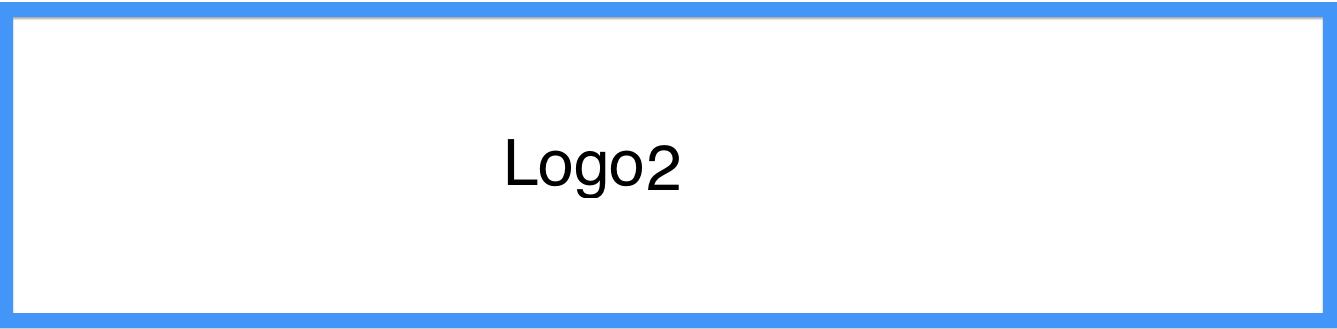
\includegraphics[width=0.3\textwidth,angle=0]{abb/logo2}
% \caption[Beschreibung]{Beschreibung}
%\label{fig:Beschreibung}
%\end{figure}

% Beispiel: Referenz auf Abbildung
Abbildung~\ref{fig:Beschreibung} [S.\pageref{fig:Beschreibung}]

% Beispiel: Tabelle 
\begin{center}
  \begin{tabular}{ | l | c | }
    \hline
    Überschrift 1 & Überschrift 2 \\ \hline \hline
    Info 1 & Info 2 \\ \hline
    Info 3 & Info 4 \\
    \hline
  \end{tabular}
\end{center}


% Beispiel für Quellcode Listings
\lstset{language=xml}
\begin{lstlisting}[frame=htrbl, caption={Die Datei {\tt data-config.xml} dient als Beispiel für XML Quellcode}, label={lst:dataconfigxml}]
<dataConfig>
  <dataSource type="JdbcDataSource" 
              driver="com.mysql.jdbc.Driver"
              url="jdbc:mysql://localhost/bms_db"
              user="root" 
              password=""/>
  <document>
    <entity name="id"
        query="select id, htmlBody, sentDate, sentFrom, subject, textBody
        from mail">
    <field column="id" name="id"/>
    <field column="htmlBody" name="text"/>
    <field column="sentDate" name="sentDate"/>
    <field column="sentFrom" name="sentFrom"/>
    <field column="subject"  name="subject"/>
    <field column="textBody" name="text"/>
    </entity>
  </document>
</dataConfig>
\end{lstlisting}

\lstset{language=java}
\begin{lstlisting}[frame=htrbl, caption={Das Listing zeigt Java Quellcode}, label={lst:result2}]
/* generate TagCloud */
Cloud cloud = new Cloud();
cloud.setMaxWeight(_maxSizeOfText);
cloud.setMinWeight(_minSizeOfText);
cloud.setTagCase(Case.LOWER);
	    
/* evaluate context and find additional stopwords */
String query = getContextQuery(_context);
List<String> contextStoplist = new ArrayList<String>();
contextStoplist = getStopwordsFromDB(query);
	    
/* append context stoplist */
while(contextStoplist != null && !contextStoplist.isEmpty())
  _stoplist.add(contextStoplist.remove(0));
	    
/* add cloud filters */
if (_stoplist != null) {
  DictionaryFilter df = new DictionaryFilter(_stoplist);
  cloud.addInputFilter(df);
}
/* remove empty tags */
NonNullFilter<Tag> nnf = new NonNullFilter<Tag>();
cloud.addInputFilter(nnf);

/* set minimum tag length */
MinLengthFilter mlf = new MinLengthFilter(_minTagLength);
cloud.addInputFilter(mlf);

/* add taglist to tagcloud */
cloud.addText(_taglist);

/* set number of shown tags */	    
cloud.setMaxTagsToDisplay(_tagsToDisplay);
\end{lstlisting}


% Beispiel für Formeln
Die Zuordnung aller möglichen Werte, welche eine Zufallsvariable annehmen kann nennt man \emph{Verteilungsfunktion} von $X$.

\begin{quotation}
Die Funktion F: $\mathbb{R} \rightarrow$ [0,1] mit $F(t) = P (X \le t)$ heißt Verteilungsfunktion von $X$.\footnote{Konen, vgl.~\cite{wk05}~[S.55]}
\end{quotation}

\begin{quotation}
Für eine stetige Zufallsvariable $X: \Omega \rightarrow \mathbb{R}$ heißt eine integrierbare, nichtnegative reelle Funktion $w: \mathbb{R} \rightarrow \mathbb{R}$ mit $F(x) = P(X \le x) = \int_{-\infty}^{x} w(t)dt$ die \emph{Dichte} oder \emph{Wahrscheinlichkeitsdichte} der Zufallsvariablen $X$.\footnote{Konen, vgl.~\cite{wk05}~[S.56]}
\end{quotation}











\onecolumn
% einfacher Zeilenabstand
\singlespacing
% Literaturliste soll im Inhaltsverzeichnis auftauchen
\newpage
\addcontentsline{toc}{section}{Literaturverzeichnis}
% Literaturverzeichnis anzeigen
\renewcommand\refname{Literaturverzeichnis}
\bibliography{Hauptdatei}

%% Index soll Stichwortverzeichnis heissen
% \newpage
% % Stichwortverzeichnis soll im Inhaltsverzeichnis auftauchen
% \addcontentsline{toc}{section}{Stichwortverzeichnis}
% \renewcommand{\indexname}{Stichwortverzeichnis}
% % Stichwortverzeichnis endgueltig anzeigen
% \printindex

\onehalfspacing
% evtl. Anhang
\newpage
\addcontentsline{toc}{section}{Anhang}
\fancyhead[L]{Anhang} %Kopfzeile links
\subsection*{Anhang}\label{anhang}

%
% ---- Bibliography ----
%
\begin{thebibliography}{99}
	%
	\bibitem {wiki_jpa}
	Wikipedia
	\url{https://en.wikipedia.org/wiki/Java_Persistence_API}, 07/16/2015
	\bibitem {wiki_java_ee}
	Java Platform, Enterprise Edition
	Wikipedia
	\url{https://en.wikipedia.org/wiki/Java_Platform,_Enterprise_Edition}, 07/16/2015
	\bibitem {lucene_apache_org}
	Lucene Website
	\url{https://lucene.apache.org/core/}, 07/16/2015
	\bibitem {lucene_basic_concepts}
	Lucene Tutorial
	\url{http://www.lucenetutorial.com/basic-concepts.html}, 07/20/2015
	
	
\end{thebibliography}


% Eidesstattliche Erklärung
\addcontentsline{toc}{section}{Eidesstattliche Erklärung}
\section*{Erklärung}

\begin{verbatim}

\end{verbatim}

\noindent
\begin{LARGE}Erklärung zur Bachelorarbeit\end{LARGE}
\begin{verbatim}


\end{verbatim}
Ich versichere, die von mir vorgelegte Arbeit selbstständig verfasst zu haben. Alle Stellen, die wörtlich oder sinngemäß aus veröffentlichten oder nicht veröffentlichten Arbeiten anderer entnommen sind, habe ich als entnommen kenntlich gemacht. Sämtliche Quellen und Hilfsmittel, die ich für die Arbeit benutzt habe, sind angegeben. Die Arbeit hat mit gleichem Inhalt bzw. in wesentlichen Teilen noch keiner anderen Prüfungsbehörde vorgelegen.



\begin{displaymath}
% use packages: array
\begin{array}{ll}
Unterschrift:~~~~~~~~~~~~~~~~~~~~~~~~~~~~~~~~~~~~~~~~~~
& Ort, Datum:~~~~~~~~~~~~~~~~~~~~~~~~~~~~~~~~~~~~~~~~~~
\end{array}
\end{displaymath}


% leere Abschlussseite
\newpage
\thispagestyle{empty} % erzeugt Seite ohne Kopf- / Fusszeile
\section*{ }

\end{document}